\documentclass[red,slidestop,notes,compress,mathserif]{beamer}

%\usepackage{beamerthemesplit}
\setbeamertemplate{navigation symbols}{}
\setbeamertemplate{note page}[plain]

\usetheme{Boadilla}
\usepackage{wasysym}
\usefonttheme{professionalfonts} % using non standard fonts for beamer
\usefonttheme{serif} % default family is serif
\usepackage{fontspec}

\usepackage{fontspec}
\newfontfamily\greekfont[Mapping=tex-text]{DejaVu Serif}
\setmainfont{Liberation Serif}


\title[ΕΜΠ, Αθήνα]{Σχεδιασμός και υλοποίηση μηχανισμών pipe και fork σε unikernels} 
\author[X. Μάινας]{Μάινας Χαράλαμπος
\vspace{.75em}
\\
Επιβλέπων: Γεώργιος Γκούμας}
\date{Μάρτιος 2019}
\logo{
\includegraphics[scale=0.05]{figures/ntua_logo.pdf}
\includegraphics[scale=0.16]{figures/cslab_logo.pdf}}

\institute[CSLab, ΕΜΠ]{%High-Performance Systems and Interconnects (HPSI),\\
Εργαστήριο Υπολογιστικών Συστημάτων \\Σχολή Ηλεκτρολόγων Μηχανικών και Μηχανικών Υπολογιστών\\Εθνικό Μετσόβιο Πολυτεχνείο\\
%Github: \url{http://github.com/{HPSI,ananos}}\\
WWW: \url{http://cslab.ece.ntua.gr/research/}\\

\includegraphics[width=1.5cm]{figures/ntua_logo.pdf}

\includegraphics[width=3.5cm]{figures/cslab_logo.pdf}\\
%\includegraphics[angle=-90,width=4.0cm]{figs/hrakleitos.pdf}\\
}


\newcommand{\ta}{\insertframenumber}

\AtBeginSubsection[]
{
  \begin{frame}
  \frametitle{Επισκόπηση}
  \tableofcontents[currentsection,currentsubsection]
  \end{frame}
}
\begin{document}


\frame{\titlepage}
\section{Εισαγωγή}
\subsection{Unikernels}

\begin{frame}
\frametitle{Εισαγωγή}
\begin{block}{Unikernels}
Εξειδικευμένες εικόνες μηχανές, με ένα μοναδικό χώρο διευθύνσεων, τα οποία κατασκευάζονται χρησιμοποιώντας library operating systems
\end{block}
\begin{block}{Αναλύοντας τον ορισμό}
\begin{itemize}
\item Εξειδικευμένες: κάθε unikernel περιέχει μία και μόνο εφαρμογή και έχει χτιστεί με σκοπό την υποστήριξη μόνο αυτής.
\item Μοναδικός χώρος διευθύνσεων: δεν υπάρχει διαχωρισμός kernel space και user space.
\item library operating systems: λειτουργικά συστήματα που παρέχουν τις υπηρεσίες που υποστηρίζουν (π.χ. networking) σε μορφή βιβλιοθηκών, οι οποίες μπορούν να χρησιμοποιηθούν (link) από τις εφαμρογές.
\end{itemize}
\end{block}
\end{frame}

\begin{frame}
\frametitle{Typical OS vs unikernel}
\begin{figure}
\center
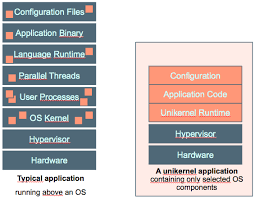
\includegraphics{figures/unikernel_vs_os.png}
\end{figure}
\end{frame}

\begin{frame}
\frametitle{Χαρακτηριστικά των unikernels}
\begin{block}{Πλεονεκτήματα}
\begin{itemize}
\item Γρήγοροι χρόνοι εκκίνησης
\item Μικρό memory footprint
\item Περισσότερη ασφάλεια
\end{itemize}
\end{block}
\begin{block}{Μειονεκτήματα}
	%%TODO: prepei na to ksanadw auto to kommati
\begin{itemize}
\item Οι εφαρμογές χρειάζονται porting
\item Πολλές βιβλιοθήκες μπορεί να μην υποστηρίζονται
\item Πολλά components των OSes μπορεί να μην υποστηρίζονται (single process)
\end{itemize}
\end{block}
\end{frame}

\subsection{Unikernel frameworks}

\begin{frame}
\frametitle{Unikernel frameworks}
	\begin{block}{Rumprun}
		\begin{itemize}
			\item Είναι βασισμένο στο NetBSD και συγκεκριμένα στα rump kernels 
			\item POSIX friendly
			\item Υποστήριξη για threads, filesystem
			\item Υποστηρίζει πολλές γλώσσες
			\item Πολλές εφαρμογές έτοιμες να εκτελεστούν σε αυτό
		\end{itemize}
	\end{block}
\end{frame}
\begin{frame}
\frametitle{Unikernel frameworks}
	\begin{block}{OSv}
		\begin{itemize}
			\item Είναι φτιαγμένο από την αρχή, με στόχο να εκτελείται στο cloud
			\item POSIX compatible
			\item Υποστήριξη για threads, filesystem.
			\item Υποστηρίζει πολλές γλώσσες
			\item Πολλές εφαρμογές έτοιμες να εκτελεστούν σε αυτό
			\item Από τα πιο ενεργά projects
		\end{itemize}
	\end{block}
\end{frame}
\begin{frame}
\frametitle{Unikernel frameworks}
	\begin{block}{IncludeOS}
		\begin{itemize}
			\item Είναι φτιαγμένο από την αρχή
			\item Μερικώς POSIX compatible
			\item single threaded
			\item Ταχύτατα αναπτυσσόμενο project
			\item Μόνο εφαμρογές σε C++ μπορούν να εκτελεστούν σε αυτό
		\end{itemize}
	\end{block}
\end{frame}
\begin{frame}
\frametitle{Unikernel frameworks}
	\begin{block}{MirageOS}
		\begin{itemize}
			\item Είναι φτιαγμένο από την αρχή και είναι γραμμένο σε OCaml
			\item Μόνο εφαρμογές σε OCaml μπορούν να εκτελεστούν σε αυτό
			\item Από τα πιο παλιά unikernel frameworks
		\end{itemize}
	\end{block}
	\pause
	\begin{block}{Πολλά ακόμα}
		\begin{itemize}
			\item ClickOS
			\item LKL
			\item Mini-OS, Unikraft
			\item HalVM, LING
		\end{itemize}
	\end{block}
\end{frame}

\subsection*{Rumprun}
\begin{frame}
\frametitle{Rumprun}
\begin{block}{Anykernels}
	Codebase (πυρήνα) όπου οι οδηγοί μπορούν να εξαχθούν και να ενσωματωθούν σε οποιοδήποτε μοντέλο ΛΣ
\end{block}
\begin{block}{Rump kernels}
	παρέχουν drivers του NetBSD ως φορητά εξαρτήματα με τα οποία μπορούμε να εκτελέσουμε εφαρμογές χωρίς να ναι απαραίτητη η ύπαρξη ΛΣ
\end{block}
\begin{figure}
\center
	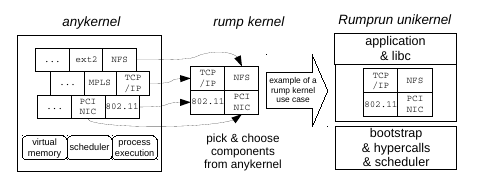
\includegraphics[scale=0.5]{figures/from_anykernel_to_rump.png}
\end{figure}
\end{frame}

\begin{frame}
\frametitle{Rumprun stack}
\begin{figure}
\center
	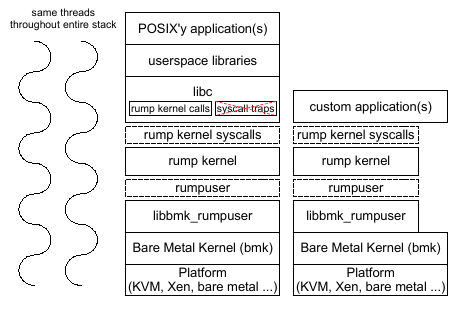
\includegraphics[scale=0.5]{figures/rumprun_stack.png}
\end{figure}
\end{frame}

\subsection{Βασική ιδέα}
\begin{frame}
\frametitle{Βασική ιδέα}
\begin{block}{Κοινό χαρακτηριστικό}
\begin{itemize}
\item Βασικό κοινό χαρακτηριστικό όλων των unikernels, είναι ότι είναι single process
\item Συνεπώς δεν υποστηρίζεται η κλήση fork, σε κανένα unikernel
\end{itemize}
\end{block}
\begin{block}{Ιδέα}
\begin{itemize}
\item Προσπαθούμε να κάνουμε τα unikernels όσο πιο πολύ POSIX friendly γίνεται
\item Θέλουμε να κρατήσουμε τα βασικά χαρακτηριστικά των unikernels
\item Αντιλαμβανόμαστε τα unikernels ως διεργασίες και το hypervisor ως λειτουργικό συτημα
\item Συνεπώς μία κλήση fork, θα οδηγούσε στη δημιουργία μίας νέας διεργασίας unikernel, αντί για μία διεργασία μέσα στο υπάρχον unikernel.
\end{itemize}
\end{block}
\end{frame}

\section{Μηχανισμός pipe}
\subsection{Γενική εικόνα}

\begin{frame}
\frametitle{Γενική εικόνα}
\begin{block}{Pipe system call}
int pipe(int fildes[2]); \\
Pipe semantics:
\begin{itemize}
\item Αν το pipe είναι άδειο, η κλήση ανάγνωσης μπλοκάρει μέχρι να προκύψουν δεδομένα
\item Αν το pipe είναι γεμάτο, η κλήση εγγραφής μπλοκάρει μέχρι να ρλρυθερωθεί χώρος
\item Αν δεν υπάρχουν ανοιχτά άκρα εγγραφής, τότε εανάγνωση στο pipe επιστρέφει 0, end of file
\item Αν δεν υπάρχουν ανοιχτά άκρα ανάγνωσης, τότε εγγραφή στο pipe επιστρέφει το error EPIPE
\end{itemize}
\end{block}
\end{frame}

\begin{frame}
\frametitle{Γενική εικόνα}
\begin{block}{Pipe σε unikernels}
Η κλήση συστήματος pipe χρησιμοποιείται από τα unikernels, όπως θα χρησιμοποιούταν από τις διεργασίες σε ένα συμβατικό ΛΣ>
\end{block}
\begin{block}{Τρία στάδια υλοποίησης}
\begin{enumerate}
\item function call (με χρήση TCP/IP sockets)
\item system call (με χρήση UDP sockets)
\item system call (με χρήση κοινής μνήμης μεταξύ εικονικών μηχανών)
\end{enumerate}
\end{block}
\end{frame}

\subsection{Πρώτο στάδιο υλοποίησης}

\begin{frame}
\frametitle{Πρώτο στάδιο υλοποίησης}
\begin{block}{function call}
\begin{itemize}
\item Προσθέτουμε στον κώδικα της εφαρμογής, το function call pipe
\item Καλώντας τη συνάρτηση δημιουργούνται δύο sockets, ένα για την αποστολή και ένα για τη λήψη δεδομένων. 
\item Τα δύο αυτά sockets επιστρέφονται και μπορούν να χρησιμοποιηθούν αντίστοιχα
\item Η διεύθυνση του παραλήπτη, ορίζεται στον κώδικα της εφαρμογής
\item Δεν υλοποιήθηκαν όλα τα semantics του pipe 
\end{itemize}
\end{block}
\end{frame}

\subsection{Δεύτερο στάδιο υλοποίησης}

\begin{frame}
\frametitle{Δεύτερο στάδιο υλοποίησης}
\begin{block}{system call}
\begin{itemize}
\item Χρήση UDP sockets, αντί για TCP
\item Δημιουργία system call για τον πυρήνα του NetBSD
\item Δημιουργία δύο sockets, ένα για αποστολή και ένα για λήψη δεδομένων.
\item Επιστρέφονται δύο file descriptors, ένα για εγγραφή και ένα για ανάγνωση.
\item Η διεύθυνση του παραλήπτη, ορίζεται μέσω μίας κλήσης ioctl στο άκρο εγγραφής του pipe.
\item Δεν υλοποιήθηκαν όλα τα semantics του pipe 
\end{itemize}
\end{block}
\end{frame}

\subsection{Τρίτο στάδιο υλοποίησης}
\begin{frame}
\frametitle{Τρίτο στάδιο υλοποίησης}
\begin{block}{system call}
\begin{itemize}
\item Χρήση κοινής μνήμης μεταξύ των εικονικών μηχανών (ivshmem - nahanni)
\item Επιστρέφονται δύο file descriptors, ένα για εγγραφή και ένα για ανάγνωση.
\item Μόνο για unikernels που μοιράζονται τον ίδιο host
\item Υλοποιήθηκαν όλα τα semantics του pipe 
\end{itemize}
\end{block}
\end{frame}

\begin{frame}
\frametitle{Τρίτο στάδιο υλοποίησης}
\begin{block}{ivshmem}
\begin{itemize}
\item Για την κοινή μνήμη χρησιμοποιήθηκε ο μηχανισμός ivshmem - nahanni
\item Επιτρέπει την κοινή μνήμη μεταξύ δύο εικωνικών μηχανών σε QEMU
\item Πρέπει να υλοποιηθεί ένας PCI driver για τη χρήση του
\end{itemize}
\end{block}
\begin{block}{Υλοποίηση}
\begin{itemize}
\item PCI driver για το NetBSD και το rumprun
\item Pipe system call που χρησιμοποιεί την κοινή μνήμη
\end{itemize}
\end{block}
\end{frame}

\begin{frame}
\frametitle{Τρίτο στάδιο υλοποίησης}
\begin{block}{Υλοποίηση}
\begin{itemize}
\item PCI driver για το NetBSD και το rumprun
\item Pipe system call που χρησιμοποιεί την κοινή μνήμη
\end{itemize}
\end{block}
\begin{figure}
\center
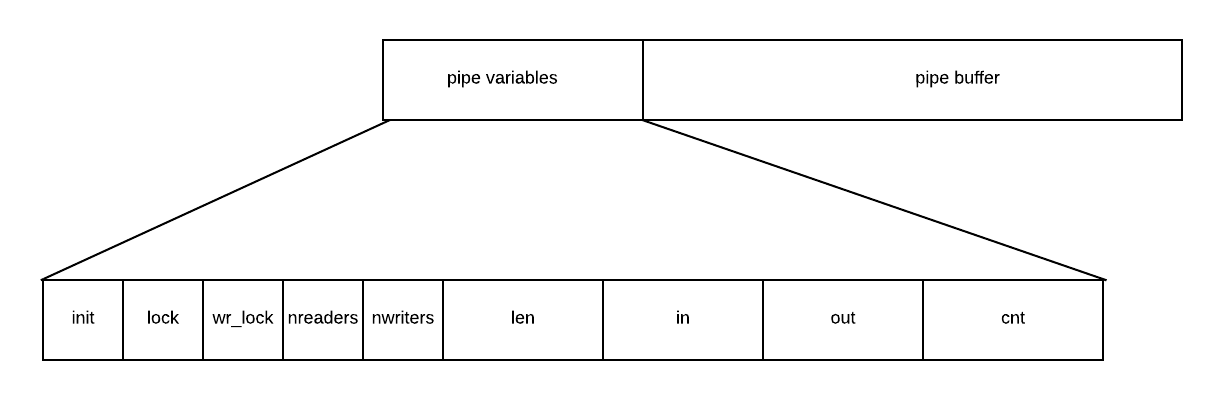
\includegraphics[scale=0.66]{figures/shared_memoery_layout.png}
\end{figure}
\end{frame}

\begin{frame}
\frametitle{Τρίτο στάδιο υλοποίησης}
\begin{columns}
\column{.4\textwidth}
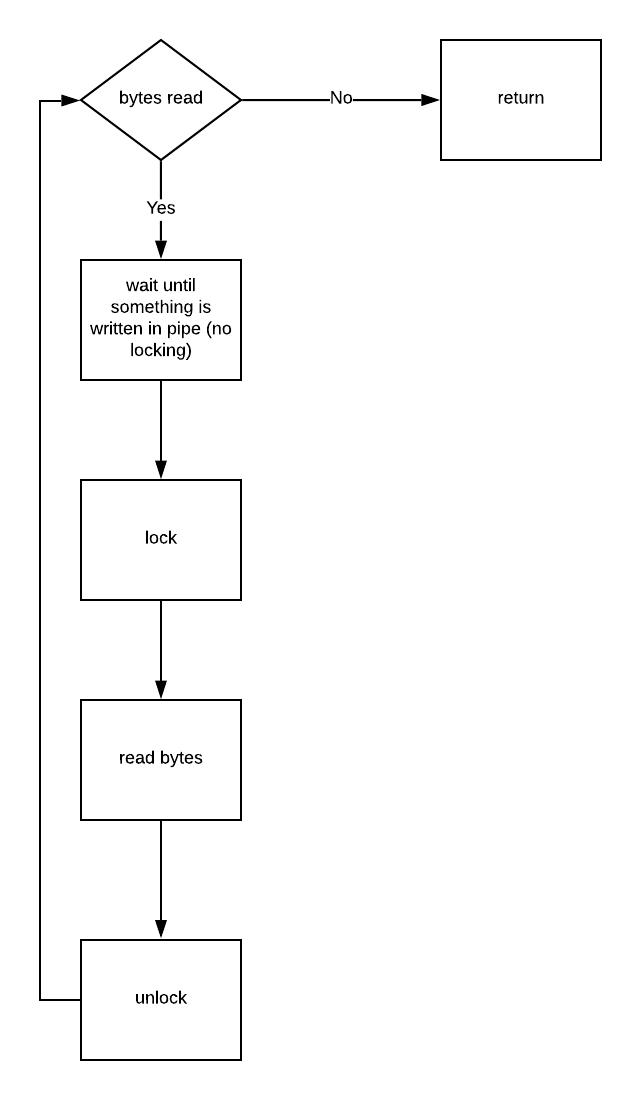
\includegraphics[scale=0.4]{figures/pipe_read.png}
\column{.4\textwidth}
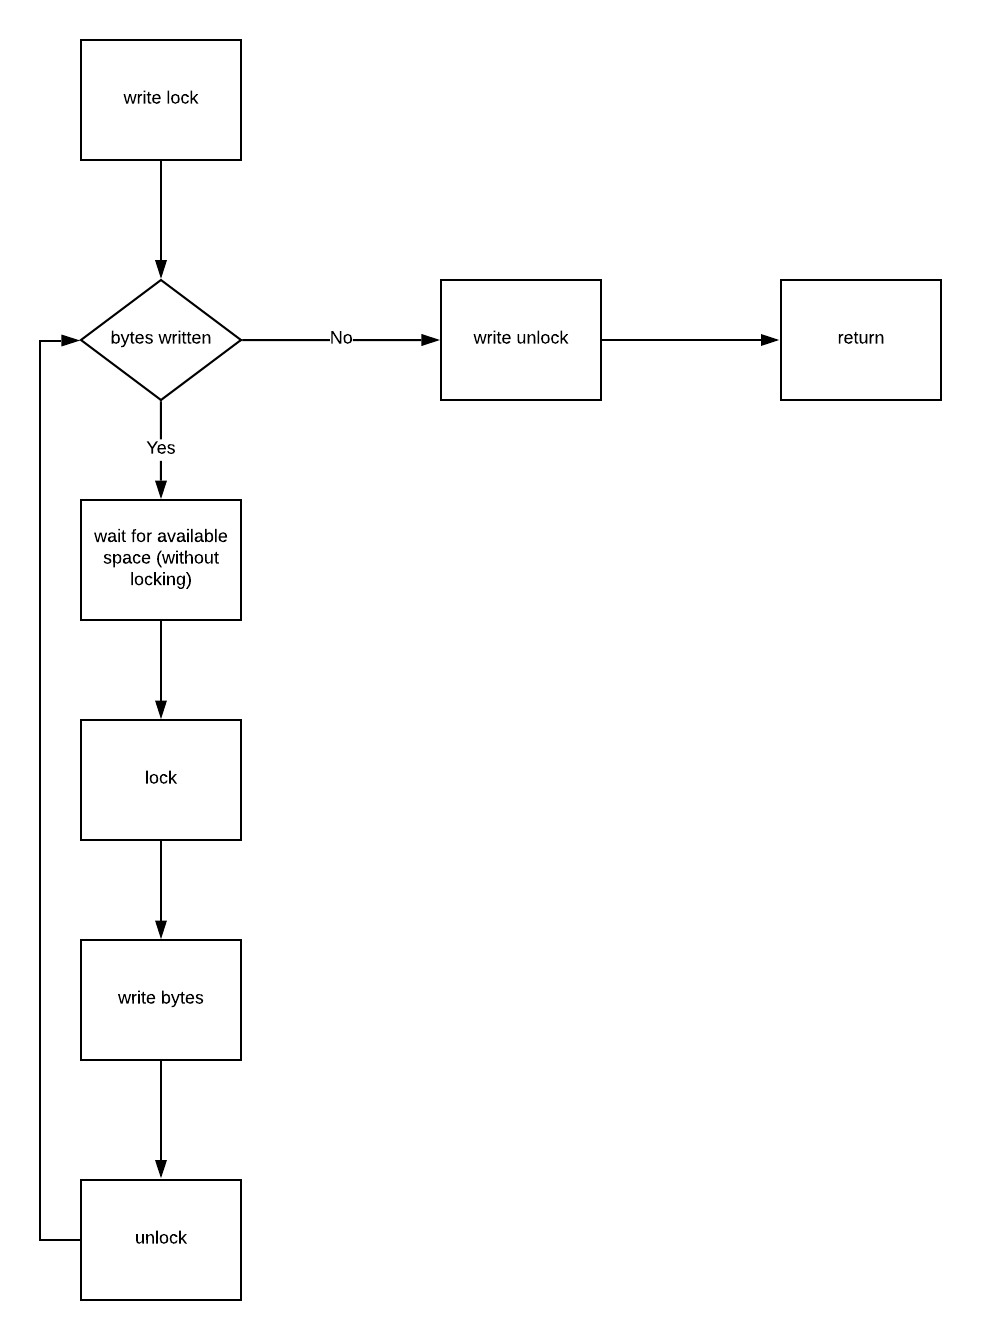
\includegraphics[scale=0.4]{figures/pipe_write.png}
\end{columns}
\end{frame}

\section{Μηχανισμός fork}
\subsection{Γενική εικόνα}
\begin{frame}
\frametitle{Γενική εικόνα}
\begin{block}{fork system call}
\begin{itemize}
\item Δημιουργία νέας διεργασίας
\item Η νέα διεργασία είναι ίδια με τη διεργασία γονέα
\item Διαχωρισμός των δύο διεργασιών με τιμή επιστροφής από την κλήση συστήματος
\item Τα ανοιχτά file descriptors της διεργασίας γονέα, διατηρούνται και στη διεργασία παιδί
\end{itemize}
\end{block}
\pause
\begin{block}{Στόχος}
Η μεταφορά της ίδιας λειτουργίας σε επίπεδο εικονικών μηχανών
\end{block}
\end{frame}

\begin{frame}
\frametitle{Γενική εικόνα}
\begin{block}{Υλοποίηση}
\begin{itemize}
\item Χρήση του μηχανισμού migration, που παρέχει το QEMU, με μικρές αλλαγές
\item hypercalls από το fork system call του rumprun
\end{itemize}
\end{block}
\begin{block}{Βήματα}
\begin{itemize}
\item Ενημέρωση των κοινών μεταβλητών του pipe (αν υπάρχει pipe)
\item Εκκίνηση διαδικασίας migration
\item Αναμονή για migration
\item Εκκίνηση νέας εικονικής μηχανής με βάση το migration file
\end{itemize}
\end{block}
\end{frame}

\begin{frame}
\frametitle{Γενική εικόνα}
\begin{figure}
\center
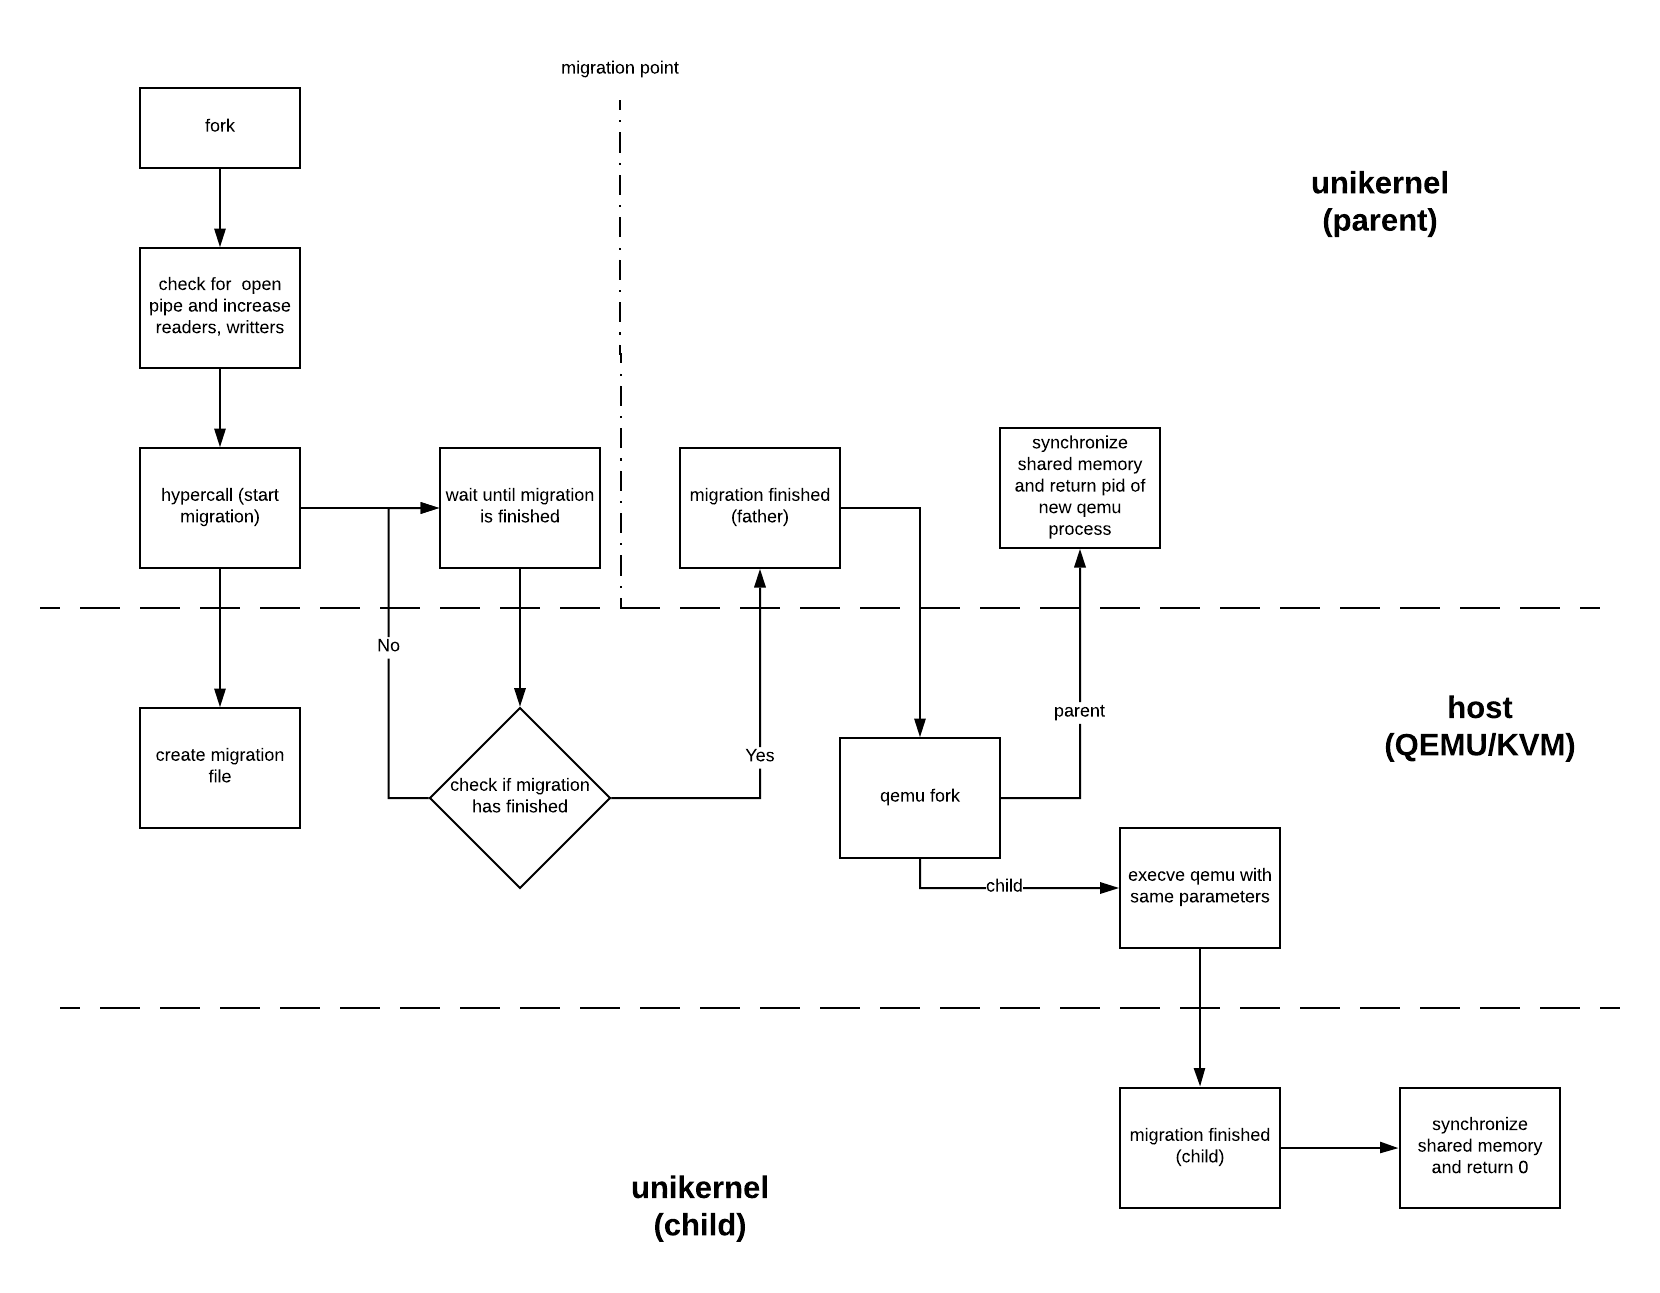
\includegraphics[scale=0.4]{figures/fork_olo.png}
\end{figure}
\end{frame}

\begin{frame}
\frametitle{Γενική εικόνα}
\begin{figure}
\center
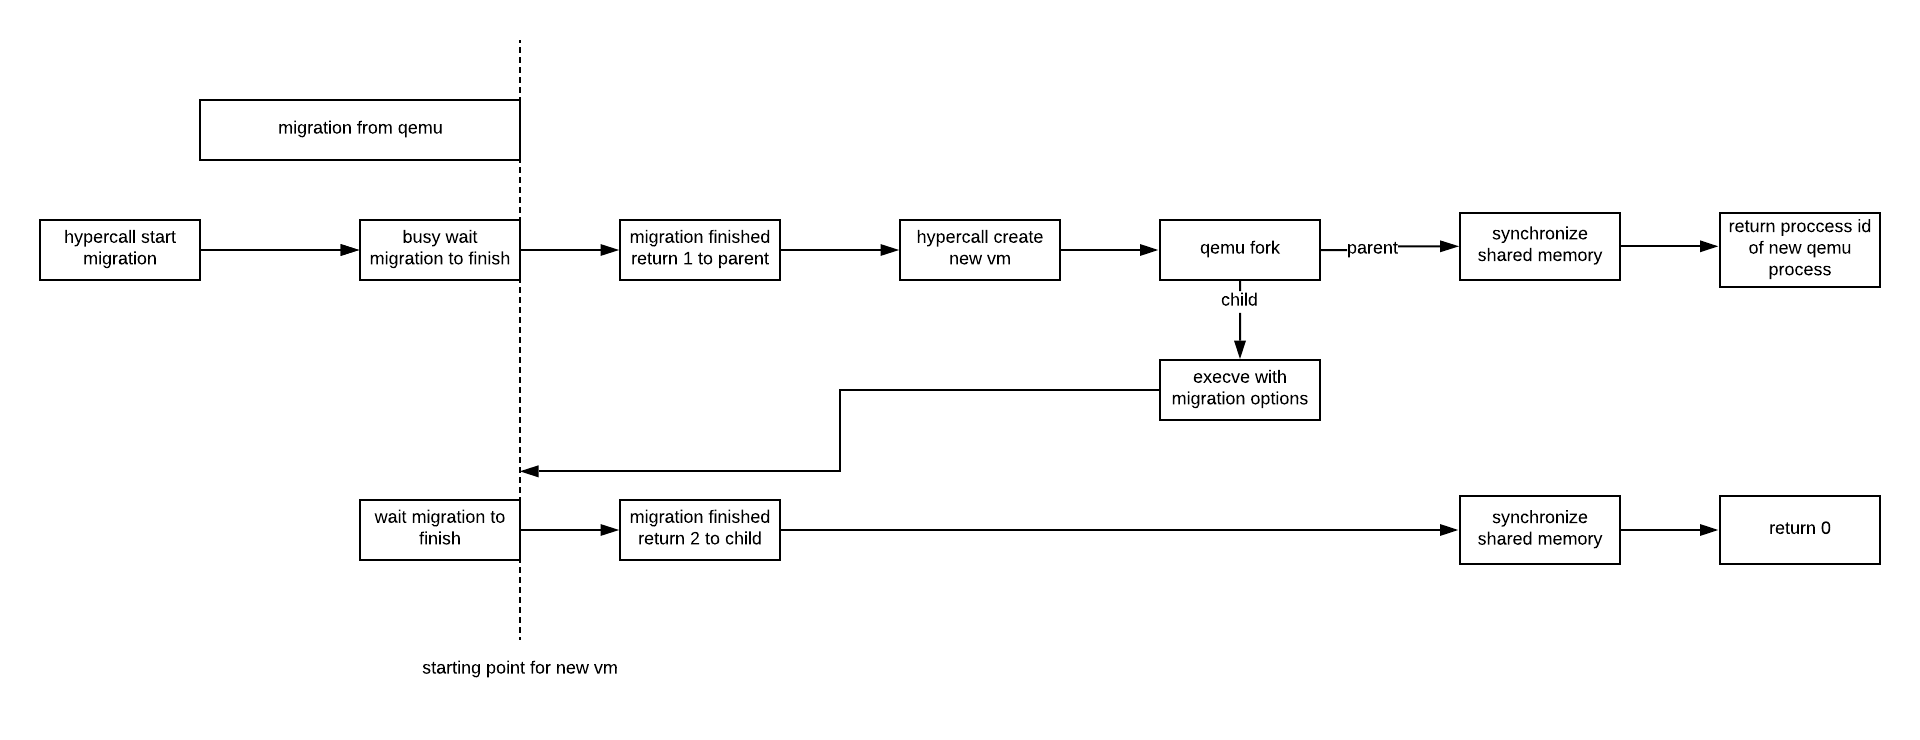
\includegraphics[scale=0.4]{figures/fork_timeline.png}
\end{figure}
\end{frame}

\subsection{Βήματα}

\begin{frame}
\frametitle{Ενημέρωση κοινών μεταβλητών στο pipe}
\begin{itemize}
\item Αν υπάρχει pipe θα πρέπει να ενημρωθούν οι κοινές μεταβλητές
\item Έλεγχος ύπαρξης pipe, μέσω των ανοιχτών file descriptors της εφαρμογής
\item Αύξηση των μετρητών ανοιχτών άκρων
\item Χάρις το migration, η εικονική μηχανή παιδί θα έχει πρόσβαση στην κοινή μνήμη
\end{itemize}
\end{frame}

\begin{frame}
\frametitle{Εκκίνηση δημιουργίας migration file}
\begin{block}{Από τη μεριά του rumprun}
Hypercall για την εκκίνηση δημιουργίας migration file
\end{block}
\begin{block}{Από τη μεριά του QEMU}
\begin{itemize}
\item Χρήση του μηχανισμού migration του QEMU
\item Δημιουργία ενος thread, που αναλαμβάνει αυτή την εργασία
\item Μικρές αλλαγές στον κώδικα του migration, ώστε να μη σταματήσει η λειτουργία της εικονικής μηχανής γονέας
\item Καθόλη τη διάρκεια του migration η εικονική μηχανή θα πρέπει να εκτελείται
\end{itemize}
\end{block}
\end{frame}

\begin{frame}
\frametitle{Αναμονή για την περάτωση του migration}
\begin{block}{Από τη μεριά του rumprun}
\begin{itemize}
\item Busy wait με συνεχή hypercalls
\item Είναι το σημείο που θα εκκινήσει τη λειτουργεία του το unikernel παιδί.
\end{itemize}
\end{block}
\begin{block}{Από τη μεριά του QEMU}
\begin{itemize}
\item Για κάθε hypercall ελέγχεται αν το migration thread εκτελείται ακόμα
\item Διατήρηση counter, για τα πόσα hypercalls γίνονται
\end{itemize}
\end{block}
\end{frame}

\begin{frame}
\frametitle{Αναμονή για την περάτωση του migration}
\begin{block}{Hypercalls counter}
\begin{itemize}
\item Με αυτόν διακρίνουμε αν πρόκειται για το παιδί ή το γονέα
\item Κάθε εικονική μηχανή στο QEMU είναι μία ξεχωριστή διεργασία, άρα διαφορετικοί counters για κάθε vm
\item Migration είναι χρονοβόρα διαδικασία, ο γονέας θα κάνει αρκετά hypercalls
\item Όταν θα εκκινήσει το παιδί το migration θα έχει ολοκληρωθεί, άρα ακριβώς ένα hypercall
\end{itemize}
\end{block}
\end{frame}

\begin{frame}
\frametitle{Αναμονή για την περάτωση του migration}
\begin{figure}
\center
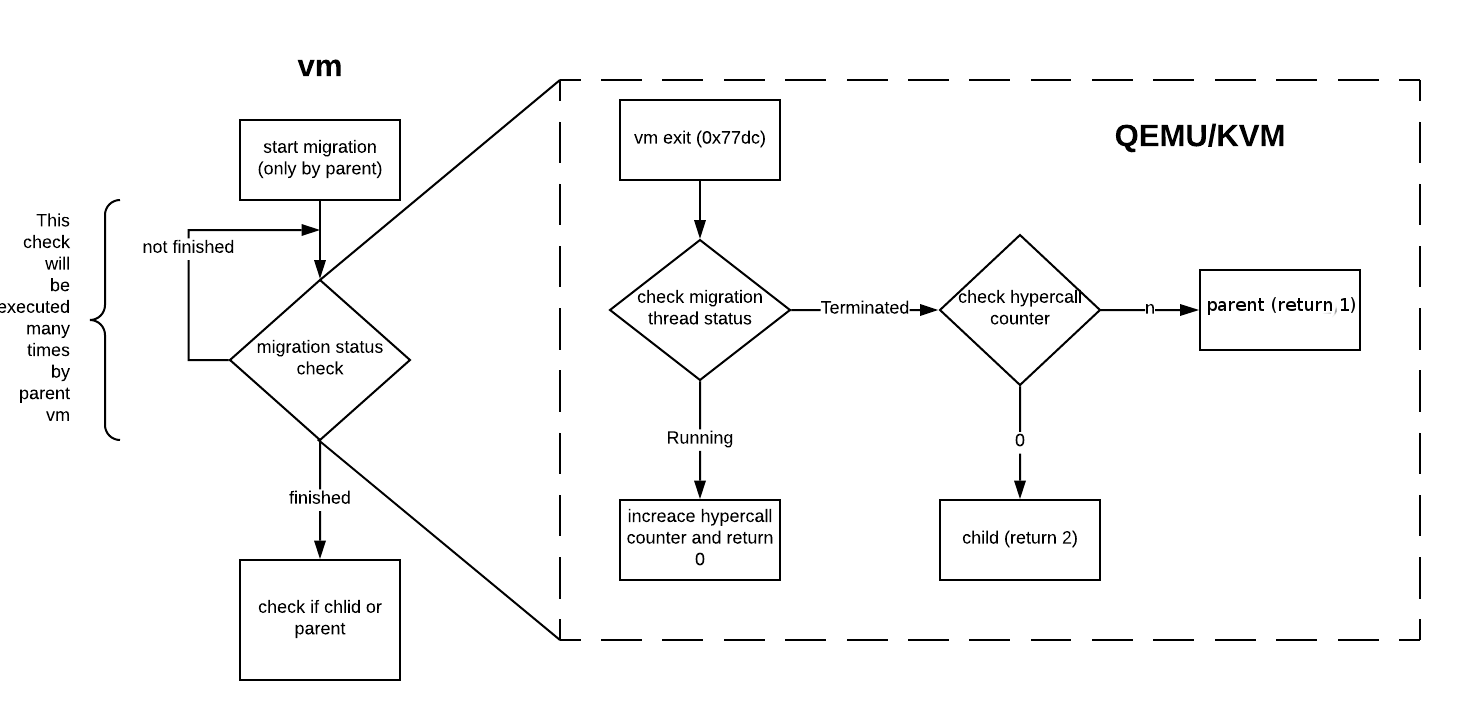
\includegraphics[scale=0.57]{figures/check_migration_status.png}
\end{figure}
\end{frame}

\begin{frame}
\frametitle{Δημιουργία νέας εικονικής μηχανής}
\begin{block}{Από τη μεριά του rumprun}
Hypercall για την εκκίνηση νέας εικονικής μηχανής
\end{block}
\begin{block}{Από τη μεριά του QEMU}
\begin{itemize}
\item fork 
\item Επιστροφή στoν γονέα το process id της νέας διεργασίας
\item Εκκίνηση νέας εικονικής μηχανής με βάση το migration file 
\end{itemize}
\end{block}
\end{frame}

\begin{frame}
\frametitle{Συγχρονισμός εικονικής μνήμης}
\begin{itemize}
\item Μόνο στην περίπτωση που χρησιμοποιείται pipe
\item Παρατηρήθηκε ότι αν το παιδί δε γράψει κάτι στην κοινή μνήμη, τότε το παιδί δεν μπορεί να διαβάσει τα δεδομένα που γράφει ο γονιός
\item Busy wait από το γονιό, να αλλάξει μία τιμή το παιδί
\item Το παιδί, απλά γράφει μία προκαθορισμένη τιμή σε μία συγκεκριμένη θέση μνήμης
\end{itemize}
\end{frame}

\subsection{Αξιολόγηση}
\begin{frame}
\frametitle{Μετρήσεις}
\begin{block}{Σύγκριση fork}
\begin{itemize}
\item Σύγκριση fork σε linux πυρήνα και του fork που δημιουργήσαμε
\item Σε ίδια έκδοση QEMU (2.11.2)
\item Linux 4.9.0-7-amd64 \#1 SMP Debian 4.9.110-3+deb9u2
\item Linux: 0.541ms, Unikernel: 137,423ms
\item Λογική η διαφορά, αλλά γιατί τόσο μεγάλη?
\end{itemize}
\end{block}
\end{frame}

\begin{frame}
\frametitle{Time for each step in fork}
\begin{figure}
\center
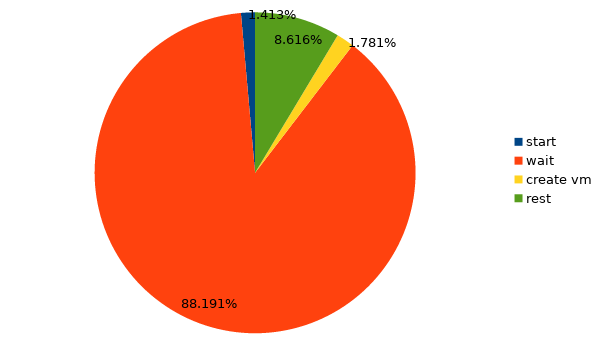
\includegraphics[scale=0.8]{figures/fork_pie.png}
\end{figure}
\end{frame}

\section*{Επίλογος}

\subsection*{Σύνοψη}

\begin{frame}
\frametitle{Σύνοψη}
Τα unikernels:
\begin{itemize}
\item αποτελούν μία αρκετά ενδιαφέρουσα τεχνολογία
\item έχουν διαφορετικούς στόχους ανάλογα με το project
\item (μερικά frameworks) προσπαθούν να είναι POSIX compatible
\item είναι από μόνα τους single process
\end{itemize}
\begin{block}{Αντιμετόπιση των unikernels ως διεργασίες}
\begin{itemize}
\item Μηχανισμός pipe για unikernels σε ίδιο και διαφορετικό host
\item Μηχανσιμός fork για unikernels σε ίδιο host
\end{itemize}
\end{block}
%\end{block}
\end{frame}

\begin{frame}
\frametitle{Μελλοντικές Επεκτάσεις}
\begin{itemize}
\item Χρήση σημάτων, ώστε να μη βασίζεται ο μηχανισμός pipe τόσο στην κοινή μνήμη
\item Επέκταση των inter-unikernel μηχανισμών επικοινωνίας (signaling, message queues)
\item Βελτίωση μηχανισμού fork, δημιουργώντας καλύτερο migration μηχανισμό
\item Επέκταση του μηχανισμού και σε άλλες πλατφόρμες.
\end{itemize}
%%Διαθέσιμο στο \url{https://github.com/HPSI/v4v}

\end{frame}
%
\begin{frame}
\frametitle{Ευχαριστώ!}
                \vfill%
\begin{columns}
        \column{.35\textwidth}
        \begin{center}
                %\vfill%
            %    \begin{block}{}
        \begin{center}
                        {\LARGE Ερωτήσεις;}
        \end{center}
             %   \end{block}
                \vfill%
                %\vfill%
        \end{center}
\end{columns}
                \vfill%
\end{frame}


\begin{frame}
\frametitle{}
                \vfill%
\begin{columns}
        \column{.35\textwidth}
        \begin{center}
                %\vfill%
            %    \begin{block}{}
             %   \end{block}
                \vfill%
                %\vfill%
        \end{center}
\end{columns}
                \vfill%
\end{frame}
%
\begin{frame}
\frametitle{}
                \vfill%
\begin{columns}
        \column{.35\textwidth}
        \begin{center}
                %\vfill%
            %    \begin{block}{}
        \begin{center}
                        {\LARGE Backup}
        \end{center}
             %   \end{block}
                \vfill%
                %\vfill%
        \end{center}
\end{columns}
                \vfill%
\end{frame}

%%\begin{frame}
%%\frametitle{Πειραματική αποτίμηση -- 2M message size vs Hypercalls}
%%\begin{columns}
%%\column{.8\textwidth}
%%\includegraphics[width=\textwidth]{figures/2M.eps}
%%\end{columns}
%%\end{frame}
%%
%%\begin{frame}
%%\frametitle{Πειραματική αποτίμηση -- Datagram scale}
%%\begin{columns}
%%\column{.8\textwidth}
%%\includegraphics[width=\textwidth]{figures/bw_dgram_scale.eps}
%%\end{columns}
%%\end{frame}
%%
%%\begin{frame}
%%\frametitle{Πειραματική αποτίμηση -- Hypercalls per message}
%%\begin{columns}
%%\column{.8\textwidth}
%%\includegraphics[width=\textwidth]{figures/mix.eps}
%%\end{columns}
%%\end{frame}
%
%\begin{frame}
%\frametitle{Πειραματική αποτίμηση -- Ποσοστό χρήσης CPU για το VM}
%\begin{columns}
%\column{.8\textwidth}
%\includegraphics[width=\textwidth]{figs/bare/lat_breakdown_domU.eps}
%\end{columns}
%\end{frame}
%
%\begin{frame}
%\frametitle{Xen2MX -- I}
%\begin{columns}
%\column{.8\textwidth}
%\includegraphics[width=\textwidth]{figs/bare/xen2mx_step1.pdf}
%\end{columns}
%\end{frame}
%
%\begin{frame}
%\frametitle{Xen2MX -- II}
%\begin{columns}
%\column{.8\textwidth}
%\includegraphics[width=\textwidth]{figs/bare/xen2mx_step2.pdf}
%\end{columns}
%\end{frame}
%
%\begin{frame}
%\frametitle{Xen2MX -- III}
%\begin{columns}
%\column{.8\textwidth}
%\includegraphics[width=\textwidth]{figs/bare/xen2mx_step3.pdf}
%\end{columns}
%\end{frame}
%
%\begin{frame}
%\frametitle{Xen2MX -- IV (Bridged)}
%\begin{columns}
%\column{.8\textwidth}
%\includegraphics[width=\textwidth]{figs/bare/xen2mx_step4.pdf}
%\end{columns}
%\end{frame}
%
%\begin{frame}
%\frametitle{Xen2MX -- ΙV (IOV)}
%\begin{columns}
%\column{.8\textwidth}
%\includegraphics[width=\textwidth]{figs/bare/xen2mx_step5.pdf}
%\end{columns}
%\end{frame}
%
%\begin{frame}
%\frametitle{Xen2MX -- IV (Xen2MX)}
%\begin{columns}
%\column{.8\textwidth}
%\includegraphics[width=\textwidth]{figs/bare/xen2mx_step6.pdf}
%\end{columns}
%\end{frame}
%

\end{document}
